%%% Document Author: J Moss
%%% Parts in LaTeX: Nicholas Dart
%%% Other Content: See authors list
%%% Document Last edit: 28.10.2014

\documentclass[11pt, article]{article}
\usepackage{a4wide}
\usepackage[english]{babel}
\usepackage{graphicx}
\usepackage{tabu}
\usepackage{textcomp}
\usepackage{fancyhdr}
\usepackage{lastpage}
\usepackage{titlesec}
\usepackage{lscape}

%%%%%%
%% Variables for version and release status
%% useage: \version
%%%%%%
\newcommand\version{0.4}
\newcommand\release{Pre-Release}

%%%%%%
%% Alias
%%%%%%
\newcommand{\sectionbreak}{\clearpage} 	%% Allways start a section on a new page

\title{ \huge CS221 Group Project \\ \Large Project Plan}
\author{
	\vspace{100pt}
	\begin{tabular}{ r || l }
		Project Team 	& jcm14, acb12, mta2, wia3, \\
						& nid21, msh4, jao14, mip34, \\
	 					& set12, daw54, anw46 \\
						& \\
		Version			& \version \\
		Status			& \release \\
		Date Published  & \today \\
		Reference 		& SE\_NO2\_MAN\_01 \\
		Department		& Computer Science \\
		Address			& Aberystwyth University \\
						& Penglais Campas \\
						& Ceredigion \\
						& SY23 3DB \\
	\end{tabular} \\
	Copyright \textcopyright Aberystwyth University 2014
	%get rid of the date on the titlepage
	\date{}
}

\pagestyle{fancy}
\fancyhf{}
\rhead{Version \version (\release)}
\rfoot{Page \thepage \hspace{1pt} of \pageref{LastPage}}
\lfoot{Aberystwyth University - Computer Science}

\begin{document}
	\setcounter{page}{1}

	\maketitle

	\tableofcontents

	\section{Introduction}
		\subsection{Purpose of this Document}
	This document has been commissioned to show our current understanding of the client's requirement specification of Reserve Plant Species Recording ("RPSR"). The project encompassing the Android Application Framework and modern Web Technologies which will provide a monitoring system for definable Areas of Interest, into a series of basic objectives and milestones. RPSR has three main component parts, an Android Application, a Website and a Database.

	The document will give a high level overview of the time line for developing and testing RPSR, an estimate of the final User Interface design, a probabilistic risk assessment, and a use case breakdown.

	The client is to read this document and confirm that their requirements have been understood and correctly interpreted by the team.
\subsection{Scope}
	The document comprises the high level design and development plan for RPSR, it should not be referred to for final software design structure. This document will follow the design specification.

	This document provides an overview of the system we have interpreted for the client, including our choice of platform (where applicable), high-level architecture and will also included a section dedicated out understanding of the target audience of the application.

	A use case diagram and corresponding table will show how the actors of the system are expected to interact with elements of the system. The document will also contain a probabilistic risk assessment for the project in full.
	This document will provide a first draft of the UI designs and are subject to alterations at a later date.\\
\subsection{Objectives}
	The objective of this document is to show our initial plan for development of RPSR, from initial UI designs and user interaction plans, through a breakdown of deliverable dates on a Gantt chart and the expected issues that could arise during development. This is as follows:
	\begin{enumerate}
	\item Provide a high level overview of system design and interaction
	\item Define the technologies used for the system
	\item Display the initial web UI
	\item Display the initial Android UI
	\item Breakdown the project into milestones
	\item Define a limited scope risk assessment for the project and the plans to mitigate the risks
	\end{enumerate}

	\section{Overview}
		\subsection{Platforms}
	\subsubsection{Android}
		The client placed a specific request for the application to run on Android devices. As yet no response has been received for a minimum version, so in keeping with more up to date releases, we will use Android API 15 (Android 4.0.3 which encompasses the vast majority of new smart phones)

	\subsubsection{LAMP Server}
		We will be using a LAMP (Linux, Apache2, MySQL, and PHP) ready server. Linux will be version Gentoo 3.12, MySQL will be version 14.14, PHP will be version 5.5.18. This will provide us with the tools ready to develop the website, and interact with the database. PHP was chosen to handle the server side processing of received data due to it being free and wide availability. The language is also covered in other modules during the project time line, meaning it will be fresh in the minds of the web team. MySQL is the most commonly used database software on web servers and is available on the university servers. 

References for Version: 
Linux: https://www.gentoo.org/
Apache2: http://httpd.apache.org/
MySQL: http://www.mysql.com/
PHP: http://php.net/
\newpage
\subsection{High Level Architecture}
	The system consists of the following high-level elements:

\subsubsection{Android Application (RPSRrec)}

	The application fulfils the following roles:\\
	\begin{tabular}{r | p{15cm}}
		FR1 & Startup of software \\
		FR1 & Allow the user to record a new visit each time they complete one \\
		FR2 & Collect information about a new visit from the user \\
		FR2 & Collect time and date information from the phone for the recordings \\
		FR3 & Allow the user to select a species from the database \\
		FR3 & Add a species to a recording \\
		FR4 & Take a photo using an Android device by capturing a new photo or selecting one from the device's library \\
		FR4 & Obtain location data from the GPS unit within and Android device to include in the recording \\
		FR4 & Allow the user to enter data for each species
		RESTATEMENT OF FUNCTIONAL REQUIREMENTS ???
		\begin{itemize}
			\item Typical location
			\item Abundance using ``DAFOR'' scale
			\item Free text comment
			\item Photo of a general scene at a typical location
			\item Photo's of the specimen
			\item Allow the user to enter a name of a new species if not currently available
		\end{itemize} \\
		FR5 & Allow the user to edit and delete local (not yet uploaded) recordings and the species data within them \\
		FR5 & These local recordings will be stored on the device storage with SQLite until they are ready to be sent to the server. \\
		FR6 & Upload the collected recordings to the remote database server whenever a network connection becomes available \\
    \end{tabular}
    
    The underlying platform of execution for this subsystem is the Android operating system.
    
\subsubsection{Website (RPSRview)}
    The website fulfills the following roles:\\    
    	\begin{tabular}{r | p{15cm}}
        	FR8 & Provide a detailed view of individual recordings \\
        	FR8 & Enable maintenance of the recordings database \\
    		FR9 & Browse and search uploaded recordings \\
        \end{tabular}
    The platform of execution of this subsystem will be the LAMP stack, making use of PHP as a scripting language and Apache2 as a HTTP server.
        
\subsubsection{Server (RPSRsrv)}
    The server plays an essential middle-man role in the system, providing persistent storage for RPSRview and RPSRrec,
    and allows for exchange of data (recordings) between the two. 

    The server fulfills the following roles:\\
    \begin{tabular}{r | p{15cm}}
        FR7 & Provide a public Web API to be used by the website and the mobile application, enabling safe HTTP access to stored recordings \\
        FR7 & Provide a MySQL database for the Web API to use as a data store \\
        FR7 & Ensure data integrity and security \\
	\end{tabular}
    The platform of execution of this subsystem will be the LAMP stack. PHP, the language, and Apache2, the HTTP server, will support the Web API, while MySQL will provide the database back-end.

\subsubsection{Interaction of Components}
    

\subsubsection{External Interface Requirements}
	\begin{tabular}{r | p{15cm}}
		EIR1 & The program should be intuitive to regular computer users \\
	\end{tabular}

\subsubsection{Performance Requirements}
	Reasonable expectations of the relevant software parts of the product: \\
	\begin{tabular}{r | p{15cm}}
		PR1 & User input should be reflected on screen within one second \\
		PR2 & Software products should run appropriately on their respective platforms:
		\begin{itemize}
			\item The app on android devices
			\item Apache and php on the web server
		\end{itemize}
	\end{tabular}

\subsubsection{Design Constraints}
	Features and limitations set forth by the user or implied by reasonable implementation: \\
	\begin{tabular}{r | p{15cm}}
		DC1 & Java must be used for all Android development by corporate policy. All Java will be built in the Android Studio IDE \\
		DC2 & The API will be developed in php and will be server-side only \\
		DC3 & Functionality of software must be shown by exploration of at least 2 reserves, with at least 2 recording visits with overlapping species recordings \\
	\end{tabular}

\subsubsection{Miscellaneous Requirements}
	\begin{tabular}{r | p{15cm}}
		MSC1 & Project will be developed in line with Group Project QA guidelines \\
	\end{tabular}

\subsection{Target Audience}
	The client stated: \\ \\
		\indent \textit{The system will be used by naturalists who are familiar with standard computer interfaces. They are concerned with accuracy of recording and they may have to operate in difficult weather conditions and in remote locations.}\\ \\

	From this we understood the users will be competent in the basic interaction with Android and Web User Interfaces. We have designed the application to have large input areas to aid in data entry when outdoors but also recognize that devices used have limited screen real estate so user interfaces should be simple and uncluttered. We have also understood the user may be entering data in areas where a real time connection to the server (RPSRsrv) is not possible so data collected should be stored until a connection can be established.\\

	The system may also be used for education purposes within a school environment and so we will also target teachers and young students. From this we understood that these users will also benefit from the above requirements since this kind of app would be used on school trips.\\
	
	We also believe the app could be beneficial in research and so the app must also look professional and efficient. \\


	\section{Use Cases}
		\subsection{Use Case Diagram}
	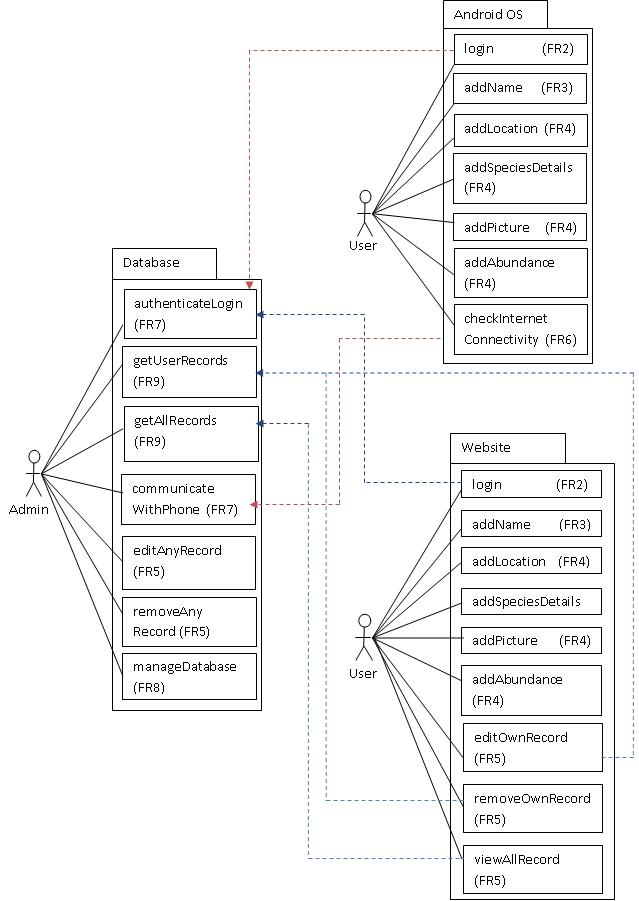
\includegraphics[scale=0.8]{useCases/useCase.png}
\subsection{Use Case Descriptions}

	\subsubsection{Android OS User}
	\begin{tabular}{| l  r | p{10cm} |}
		\hline
		FR2 & login  & User should be able to log into the application by entering a valid username\\ \hline
		FR3 & addName  & User should be able to add the name of a plant to the database \\ \hline
		FR4 & addLocation  & User should be able to add the location of a plant to the database \\ \hline
		FR4 & addSpeciesDetails  & User should be able to add a description of the plant to the database \\ \hline
		FR4 & addPicture  & User should be able to add a picture of the plant to the database \\ \hline
		FR4 & addAbundance & User should be able to record the level of abundance of the plant within the area \\ \hline
		FR6 & checkInternetConnectivity  & The application should be able to know if it is connected to the internet and is able to send records to the database. If not the data is stored in local storage \\ \hline
	\end{tabular} \\

	\subsubsection{Website user}
	\begin{tabular}{| l  r | p{10cm} |}
		\hline
		FR2 & login  & User should be able to log into the application by entering a valid username\\ \hline
		FR3 & addName & User should be able to add the name of a plant to the database \\ \hline
		FR4 & addLocation  & User should be able to add the location of a plant to the database \\ \hline
		FR4 & addSpeciesDetails  & User should be able to add a description of the plant to the database \\ \hline
		FR4 & addPicture  & User should be able to add a picture of the plant to the database \\ \hline
		FR4 & addAbundance & User should be able to record the level of abundance of the plant within the area \\ \hline
		FR5 & editOwnRecord  & User should be able to make changes to any record that they have added to the database \\ \hline
		FR5 & removeOwnRecord  & User should be able to remove any record that they have added to the database \\ \hline
		FR5 & viewAllRecord  & User should be able to view any record in the database through the website \\ \hline
	\end{tabular} \\

	\subsubsection{Admin}
	\begin{tabular}{| l  r | p{10cm} |}
		\hline
		FR7 & authenticateLogin  & The server will allow a user to log onto the application through their phone or through the website providing that the user has entered correct username and/or password. Using a database which contains details of valid usernames and passwords \\ \hline
		FR9 & getUserRecords  & When the user wants to view edit or delete records they have entered the server will need to call them from the database \\ \hline
		FR9 & getAllRecords  & The server will send information about all the records in the database to the user upon request \\ \hline
		FR9 & communicateWithPhone  & Server must be able to send and receive data from the phone of records being entered \\ \hline
		FR5 & editAnyRecord  & The website admin should be able to edit any record entered in the database by any user \\ \hline
		FR5 & removeAnyRecord  & The website admin should be able to remove any record entered into the database by any user \\ \hline
		FR8 & manageDatabase  & The database administrator will be able to log into the database and manage/maintain it \\ \hline
	\end{tabular}


	\section{User Interface Designs}
		\subsection{Android Interface}
    This section displays the envisioned design of the Android Application layout (Fig~\ref{fig:newSiteVisit}).

    \subsubsection{New Site Visit}
    
        The first thing that will be presented to the user on entry to the app will be the option to create a new visit by pushing the button provided. This will then load the Basic Information page.\\

        The user will then be prompted to input their basic information such as their name, phone number, email and site location for reference. These are to be validated by the server upon the push of the Next button. Add a species page will then be displayed to the user.\\
    
        Further fields may be required to be added at a later date due to additional requirements given by the client or by a change during further development in the design.\\
    
        There is no requirement in the spec to remember the user’s details on the app so currently the user will have to fill in their details each time they make a recording.\\
        
    \subsubsection{Adding a new species}
        
        The first input asked of the user is to select a species to record using an integrated search function. This will not only help the user find the species they are looking for, but also allow the user to add a new species to the database if required (Fig~\ref{fig:newSpecies}).\\
        
        An option to provide a GPS signal is given which will link up with the GPS in the android device to provide a location. Options are given to provide pictures of the site and specimen either from the camera or the gallery on the device. A field for adding notes will be provided that may be useful to the record (Fig~\ref{fig:editSaveSite}).\\
    
    \subsubsection{Editing and saving a site visit}
        The edit and save page provides the options to the user to view and edit the recordings made. The Edit Species link allows the user to access a list of the species pages they have added to the visit. This takes the user back to the Add a Species page to edit or delete an entry.\\
        
        Users are given the option to delete the visit which will be met with a prompt to confirm or cancel the delete.\\

        The final link is to save all recordings, giving permission to upload the data to the database at an appropriate time.\\
        
    \subsection{Web Interface}
        This section displays the envisioned design of the Website Layout.

        \subsubsection{Homepage}
           The Homepage is the first page that the user will encounter. Included in the home page, there is a central search bar to search the database for specific species, which will allow for easier searching from the start, so users can get straight into searching for a specific specimen. The navigation bar at the top remains consistent over all pages, and this will contain the main pages that the user will be accessing. The user will be able to become authenticated through the means of a form that will be contained within the header and once authenticated, be able to logout. This is essential to the user, due to there is certain features of the website that will be unavailable without authentication and this will be constant throughout the website. The main body contains a welcoming heading and text that describes the purpose of the website and information about how to use the site (Fig~\ref{fig:indexWebpage}).

        \subsubsection{Reserves}
            The reserves page will list all of the reserves in a table that will fit the width of the container that it is in. In each reserve table row, there will be a button to click to view the reserve specimens, which will take the user to the plants database page where only the reserve specimens in question will be displayed (figure). With authentication, the user will have two more buttons available within each table row. The first is the option to delete the reserve, which on click, the user will be prompted with a confirmation to ensure that there is no mistake. The second button will be the button to edit the reserve details (figure). On clicking the button, the user will be taken to a page that will allow editing to the reserve. Above the table, there will be a button to take the user to the page that will allow adding reserves. (Fig~\ref{fig:plantDbWeb}).

        \subsubsection{Add Reserve}
           The add reserves page will allow the user to add a reserve to the database, which users can then assign specimens to said reserve. There will be input fields to add reserve information such as location name and grid reference.  (Fig~\ref{fig:viewWeb}). 
        
        \subsubsection{Edit Reserve}
           The edit reserve page will hold the same input fields as the add reserve page, but the data that is held within the reserve record will be displayed already in the input fields. Once submitted, the user will be redirected to the reserves page. (Fig~\ref{fig:editWeb}).

        \subsubsection{Plant Specimens}
           The plant database provides access to the entire database using the search bar to search specimens by species name, reserve and by who created the record. The search results will be displayed within a table, with the default displaying all records. The table will only allow a limited number of specimen records at a time due to pagination which will be accessible on the sorting bar. The sorting bar will be viewable and accessible on the side of the specimen table, where it allows the user the option to order the table to their chosen criteria, where default will be by specimen ID. With the masses of records that will be held within this table, allowing the user to order by their own criteria will allow them to find the information they are looking for faster. This is where the details of the pagination and table status will be displayed. Manipulating the table of specimens will be done through AJAX to make it more dynamic, while understandably it is not a requirement, it will ensure easier and faster use.
The user will be able to clink on a link that will be held within the table to view specific specimen’s details (specimen ID). Above the table, there will be a button that will link the user to a page that will allow them to add a specimen to the database
(Fig~\ref{fig:mapWeb}).

        \subsubsection{Specimen}
     The specimen page allows the user to view specific details of the specimen that is viewed. The page will be split into two sections, where the left side will be where the details of the specimen will be contained in a vertical table. On the right side of the page container, will be the two specimen images. If the image does not exist, then there be a default image that will be displayed instead. Below the images, there is a button which will then create a pop up to display the location on a map, according to its latitude and longitude. The website will be using the GoogleMap API for this due to its ease of use and familiarity with users (Figure). If the user has been authenticated, then there will be two buttons next to the map display button. The first is the button to delete the specimen, which on click, will be presented with an alert to confirm whether the specimen should be deleted or not. The other button will be the option to edit the specimen that has been displayed, where when the user clicks on this button, it will take them to the page that will allow them to edit the specimens details  (Fig~\ref{fig:delete}).

 \subsubsection{ Add Specimen}
     This page allows the user to add a new specimen record to the database. The user will be asked to provide their individual information and specimen details such as the species name, its reserve, abundance and its latitude and longitude alongside two options to submit scene and specimen images that can be uploaded to the database upon clicking the save button.  (Fig~\ref{fig:delete}).

 \subsubsection{Edit Specimen}
        The edit specimen page is exactly like the add specimen however, the details of the specimen in question are inserted into the form values. The main difference is that the user details will not be able to be changed and the specimen reserve is also not changeable. The images will remain the same, unless the images of the specimen are updated. Once the specimen has be updated, it will be redirected to the specimen in questions page.  (Fig~\ref{fig:delete}).

    \subsection{Mockups}

        \begin{figure}
            \centering
            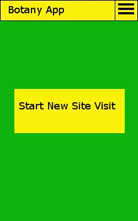
\includegraphics[scale=1]{uiDesign/botanyAppNewSiteVisit1.png}
            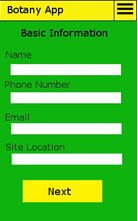
\includegraphics[scale=1]{uiDesign/botanyAppNewSiteVisit2.png}
            \caption{An example new site visit form}
            \label{fig:newSiteVisit}
        \end{figure}

        \begin{figure}
            \centering
            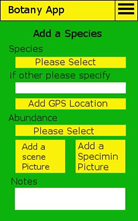
\includegraphics[scale=1]{uiDesign/botanyAppAddSpecies1.png}
            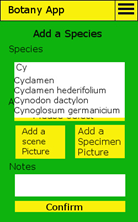
\includegraphics[scale=1]{uiDesign/botanyAppAddSpecies2.png}
            \caption{An example new species form}
            \label{fig:newSpecies}
        \end{figure}

        \begin{figure}
            \centering
            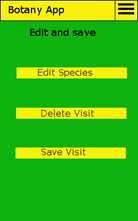
\includegraphics[scale=1]{uiDesign/botanyAppEditSaveSiteVisit.png}
            \caption{An example site/visit confirmation screen}
            \label{fig:editSaveSite}
        \end{figure}

        \begin{landscape}
            \begin{figure}
                \centering
                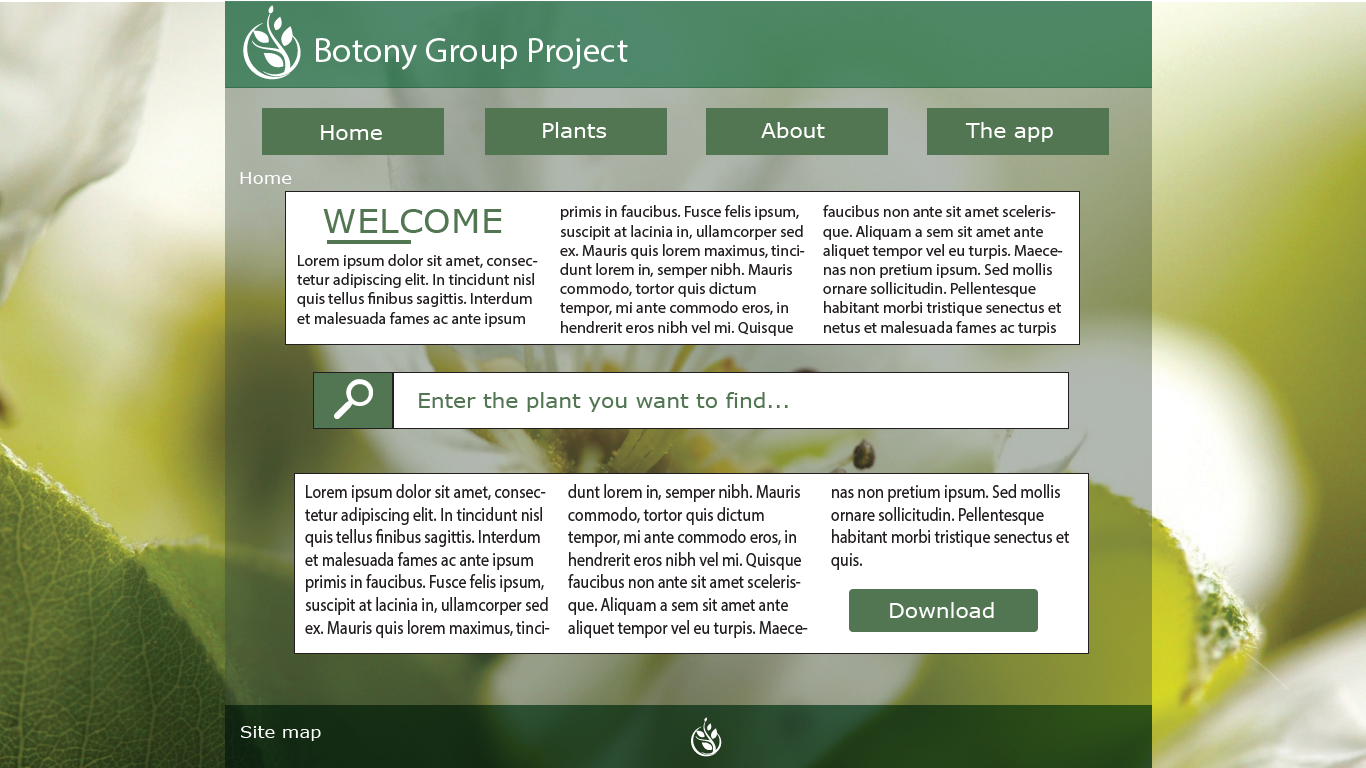
\includegraphics[scale=0.4]{uiDesign/uiwebimages/index.png}
                \caption{index.php}
                \label{fig:indexWebpage}
            \end{figure}

            \begin{figure}
                \centering
                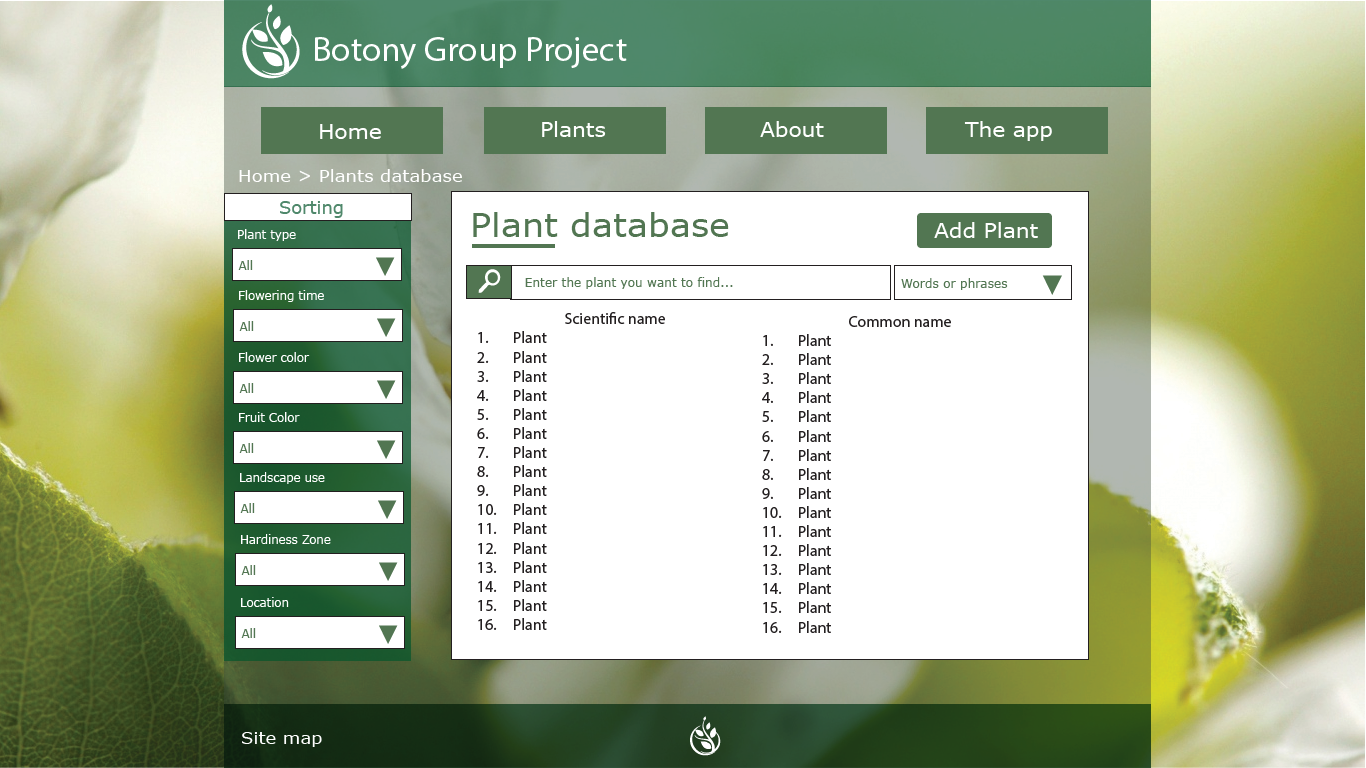
\includegraphics[scale=0.4]{uiDesign/uiwebimages/plantdb.png}
                \caption{An example of the plant database}
                \label{fig:plantDbWeb}
            \end{figure}

            \begin{figure}
                \centering
                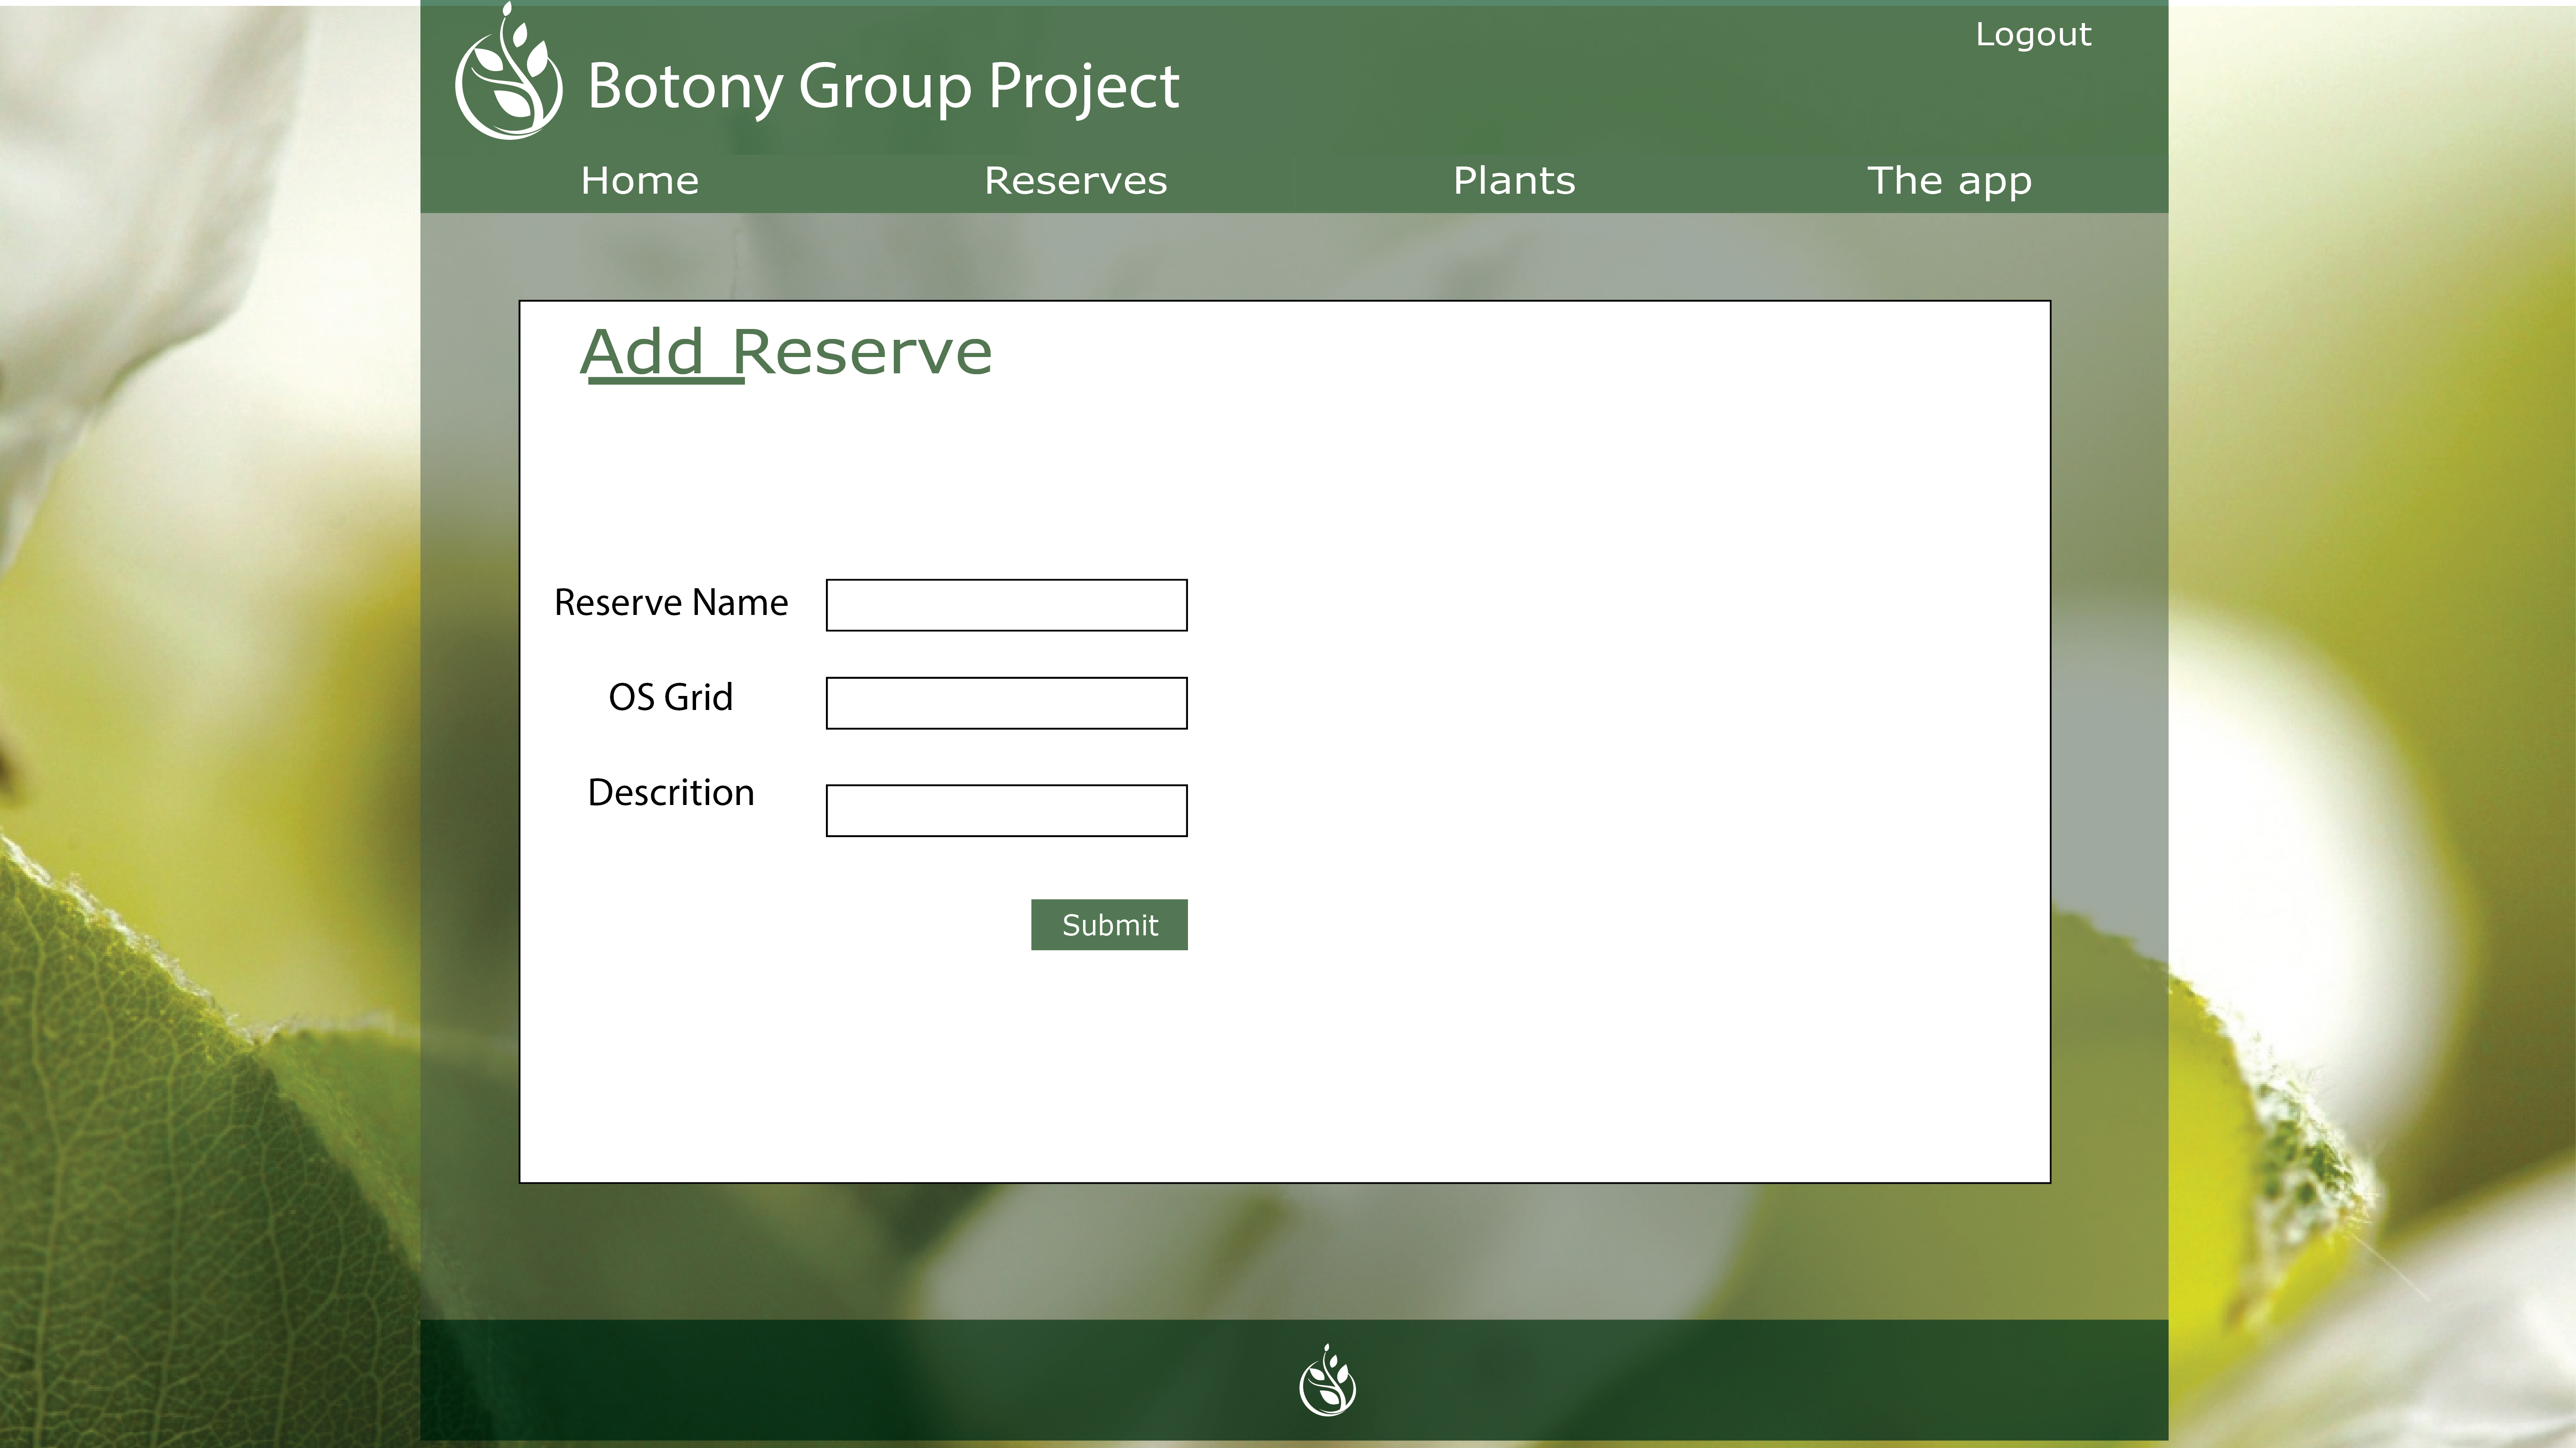
\includegraphics[scale=0.4]{uiDesign/uiwebimages/addreserve.png}
                \caption{An example plant entry in the site}
                \label{fig:viewWeb}
            \end{figure}

            \begin{figure}
                \centering
                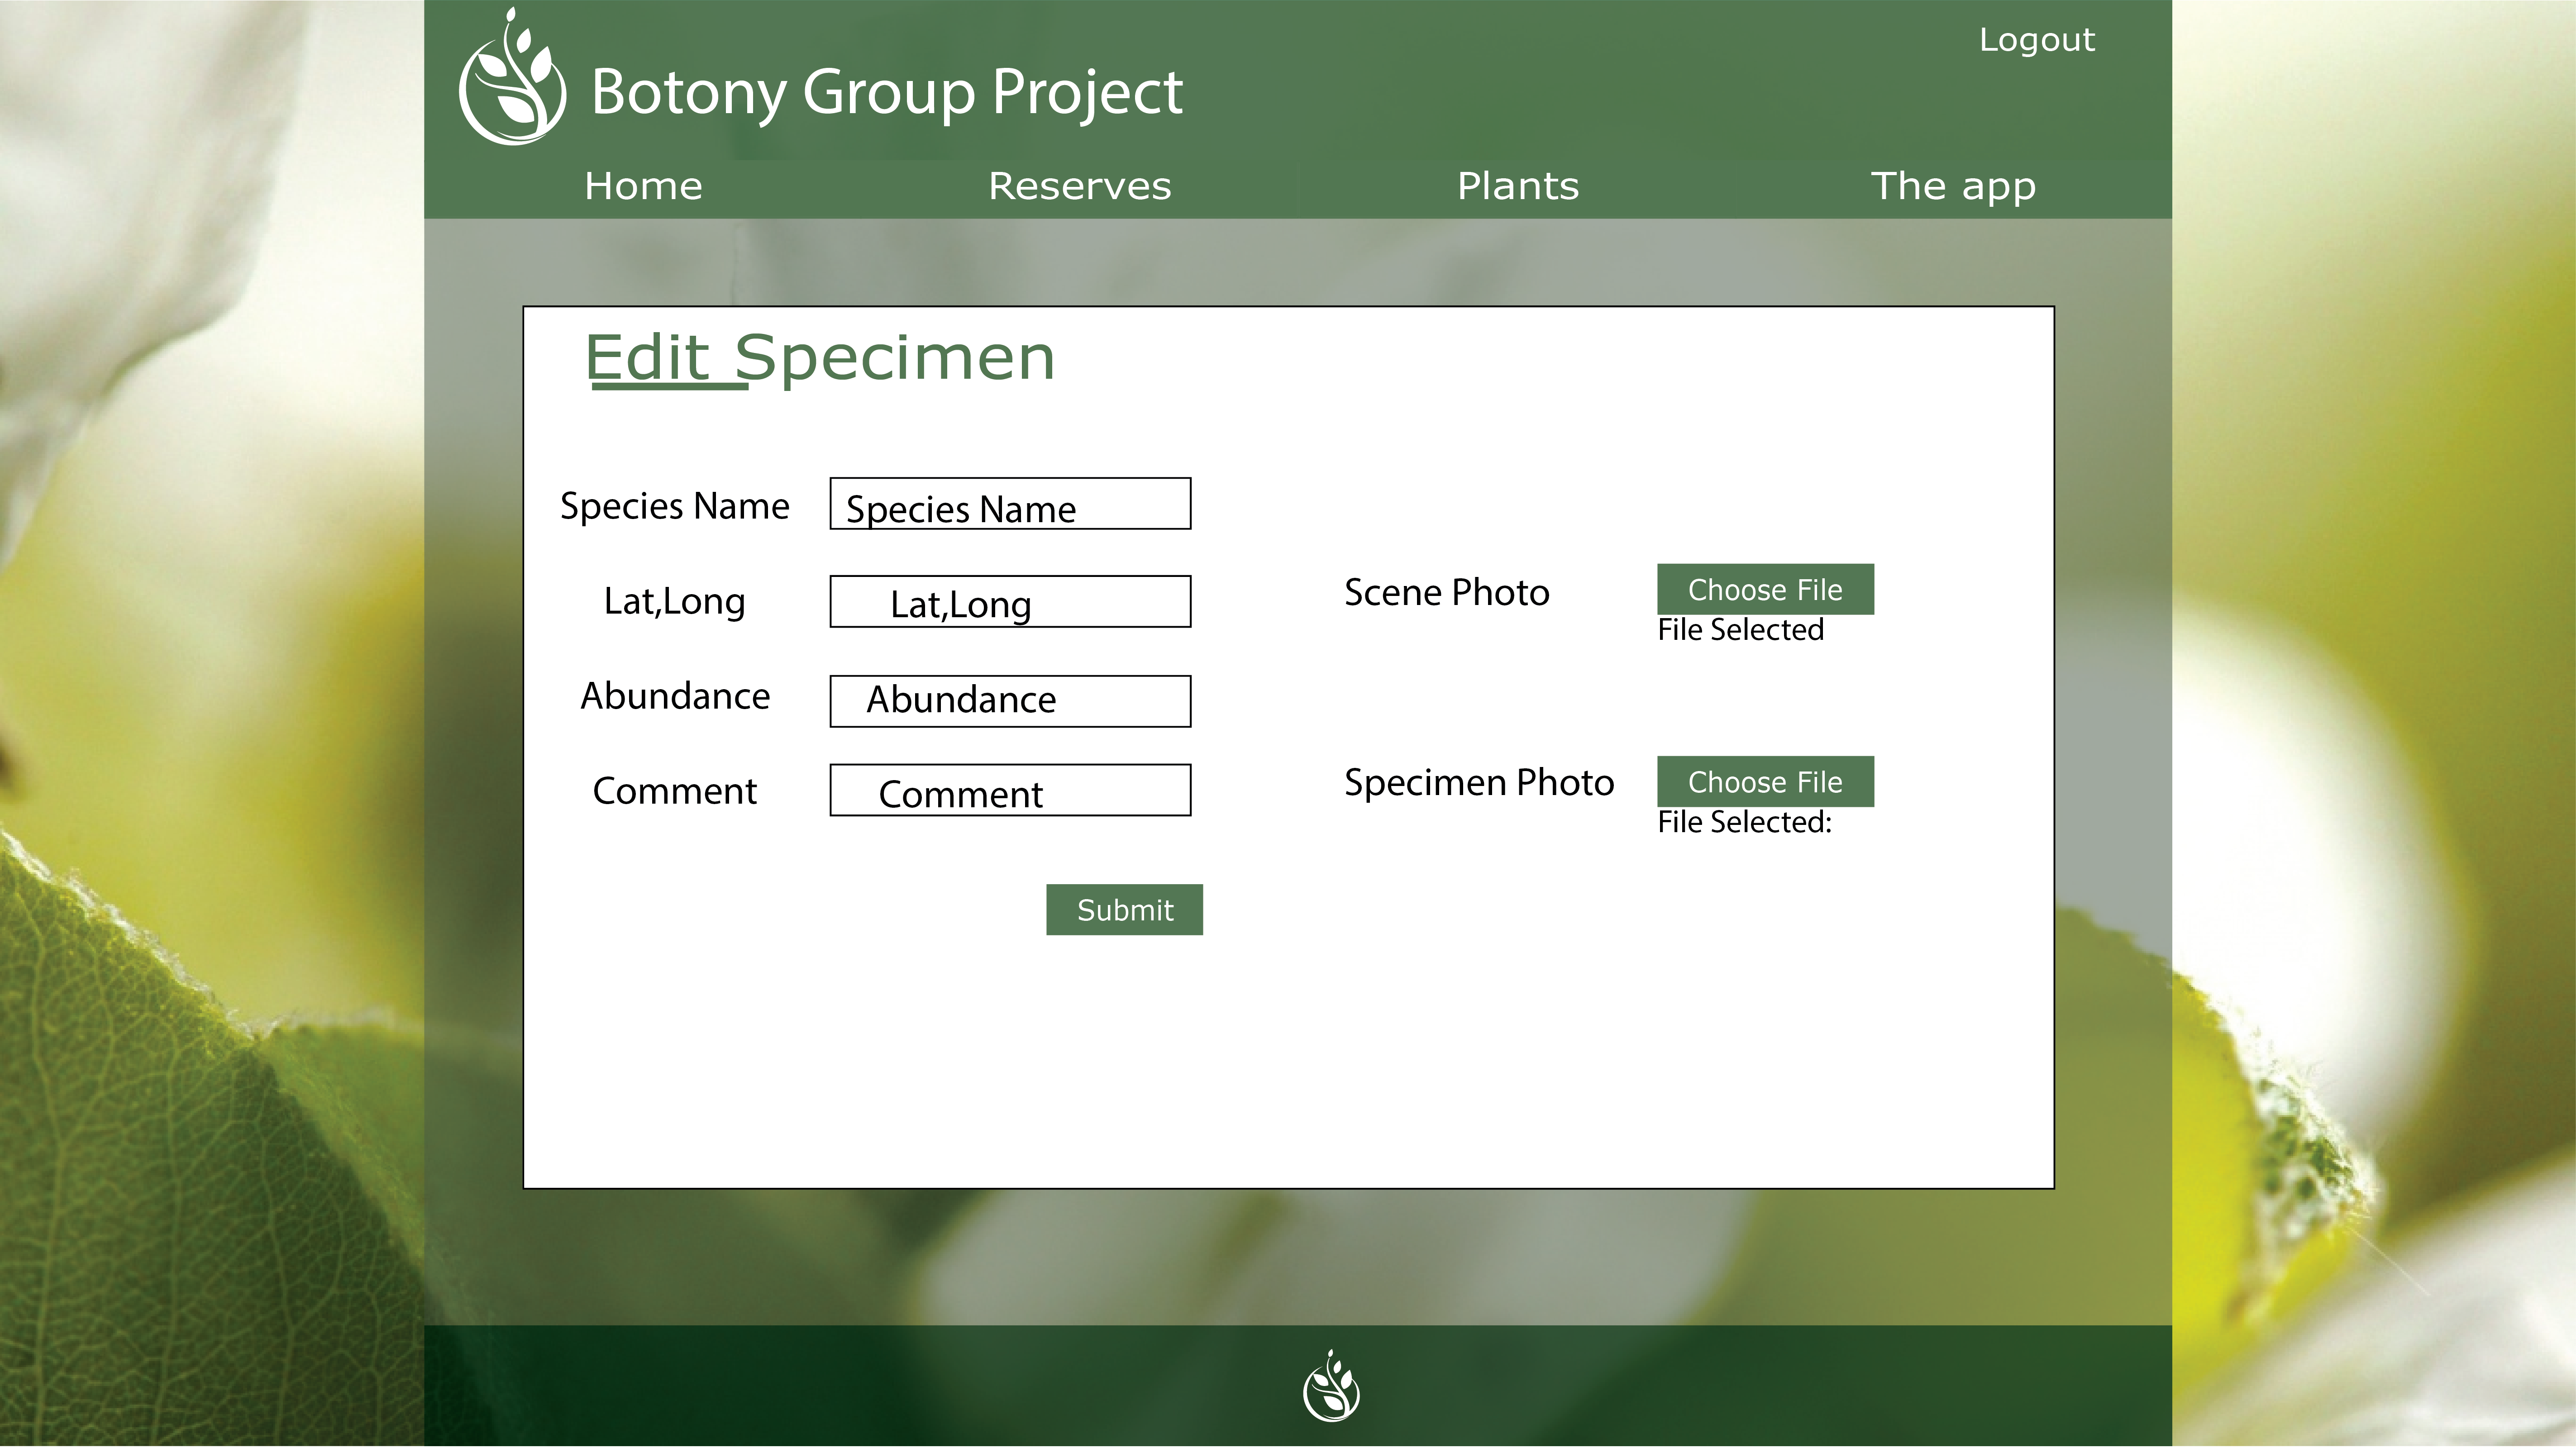
\includegraphics[scale=0.4]{uiDesign/uiwebimages/editspecimen.png}
                \caption{An example of a plant entry in edit mode}
                \label{fig:editWeb}
           \end{figure}

            \begin{figure}
                \centering
                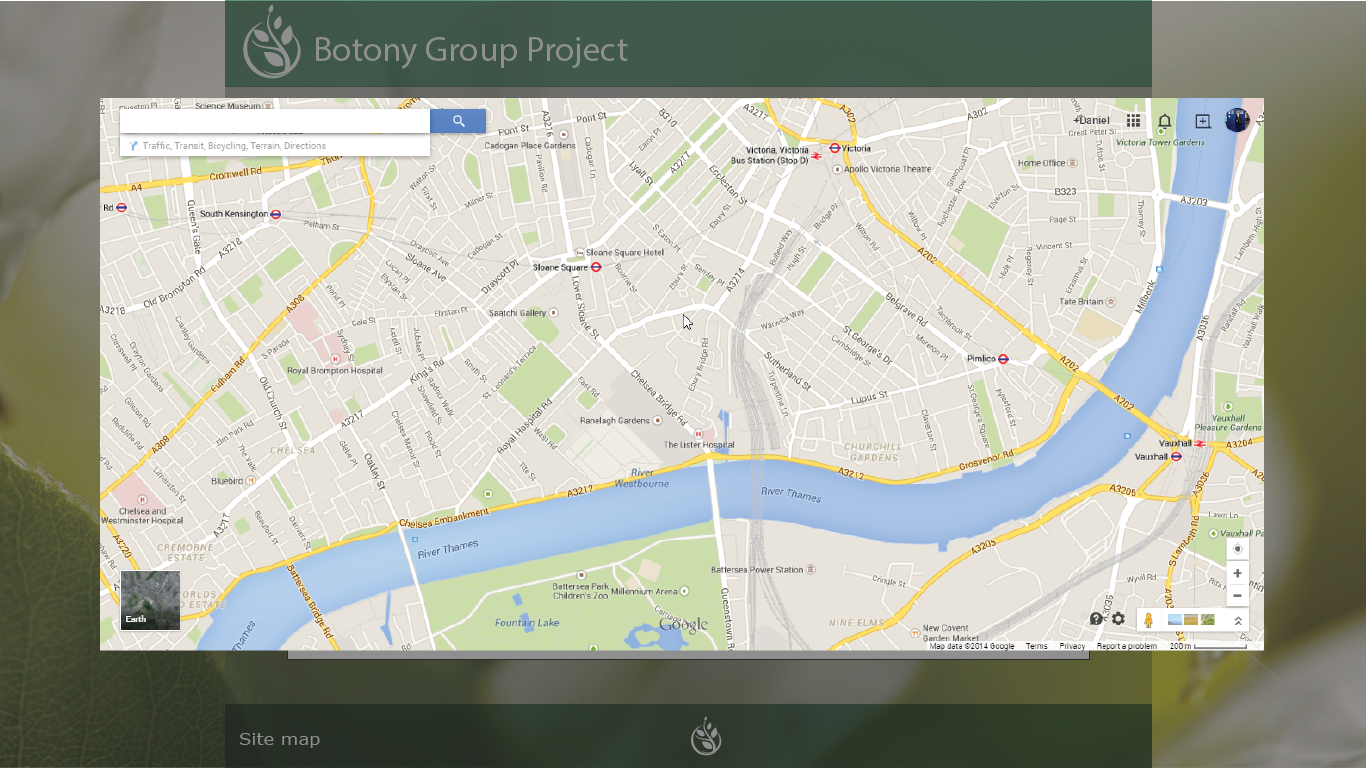
\includegraphics[scale=0.4]{uiDesign/uiwebimages/map.png}
                \caption{An example map to display recording locations}
                \label{fig:mapWeb}
            \end{figure}
        \end{landscape}

	\begin{landscape}
		\section{Gantt Chart}
			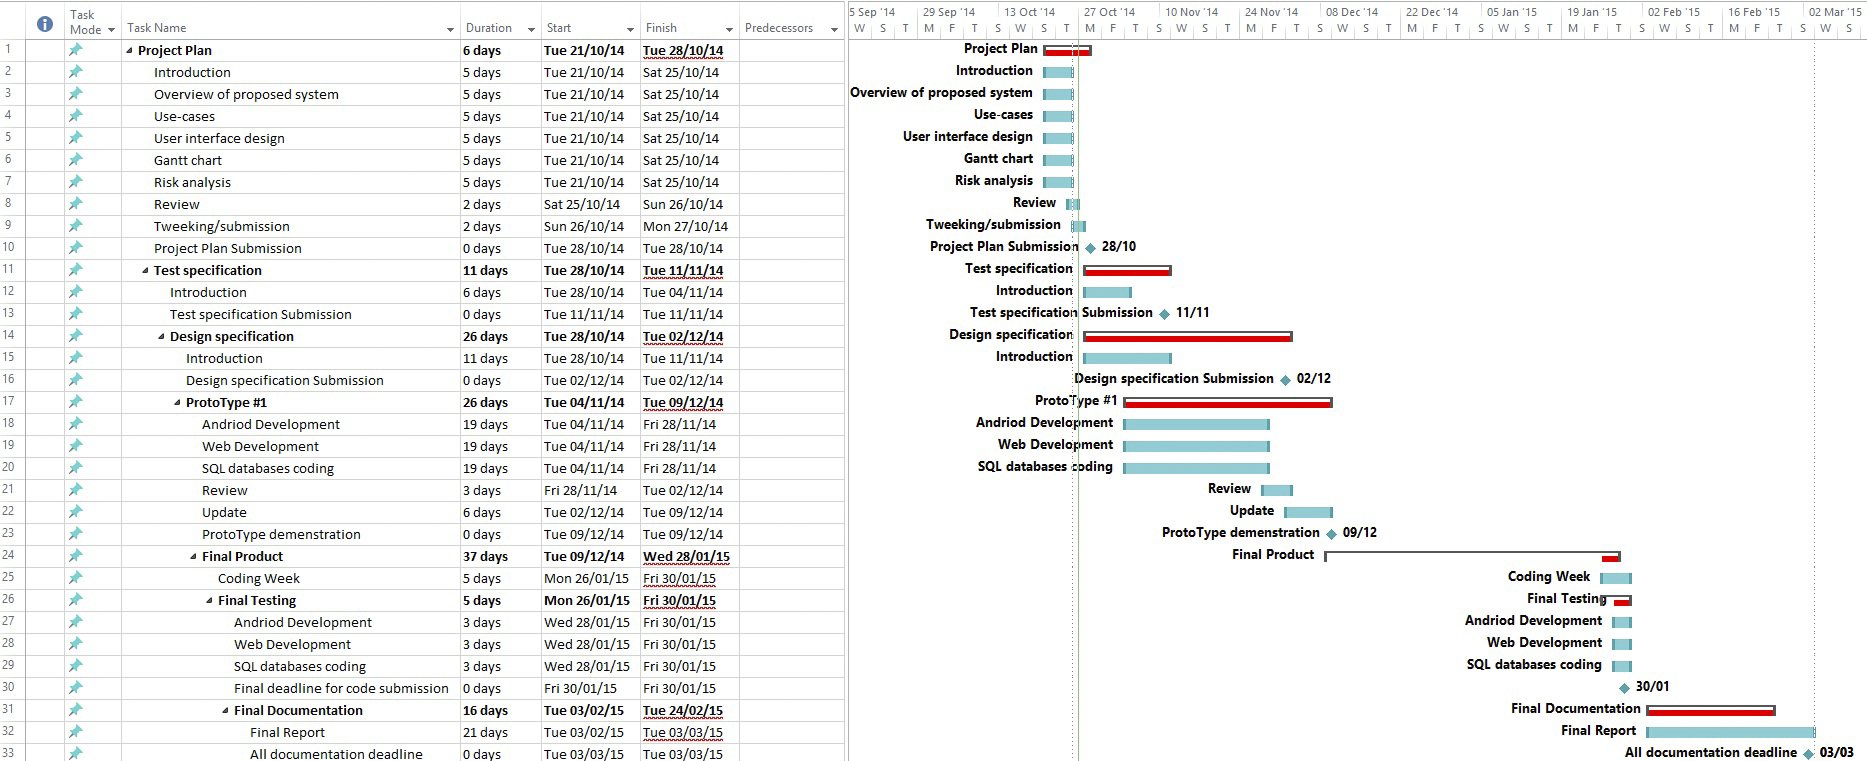
\includegraphics[scale=0.35]{ganttChart/ganttChart.png}

		\section{Risk Analysis and Mitigation}
			\newcommand\rot{rotatebox{90}}

\subsection{Onging Risk Assessments}
	\begin{tabular}[]{| p{5cm} | c | c | c | p{10cm} |}
		\hline
		\textbf{Ongoing} & \textbf{Likelyhood} & \textbf{Magnitude} & \textbf{Risk} & \textbf{Mitigation} \\ \hline \hline%\hhline{|=|=|=|=|=|}
		Planned Team Member Absence  & 2 & 2 & 4 & Meetings scheduled in advance with plenty of time for members to state if there is a problem attending. Missing member required to read minutes and report to relevant manager. \\ \hline
		Planned Project Leader Absence & 2 & 3 & 5 & Meeting to be chaired by Deputy Project Leader instead. \\ \hline
		Planned QA Manager Absence & 2 & 3 & 5 & QA Questions and Decisions to be made by Deputy QA Manager instead. \\ \hline
		Unplanned Team Member Absence  & 3 & 2 & 5 & Missing member reqired to read minutes and reprot to manager. Persistant lack of attendence to result in being carded. \\ \hline
		Unplanned Project Leader Absence & 3 & 3 & 9 & "Persistant lack of attendence to result in Deputy taking over\\ \hline
		Unplanned QA Manager Absence & 3 & 3 & 9 & "Persistant lack of attendence to result in Deputy taking over\\ \hline
		Github Downtime & 1 & 2 & 2 & Local copies to be used. \\ \hline
		Github Failure & 1 & 3 & 3 & Use backup to host locally. \\ \hline
		Long term illness & 1 & 3 & 3 & "Member to report to relevant manager in advance\\ \hline
		Member dropout & 1 & 4 & 4 & "Member to report to relevant manager in advance\\ \hline
	\end{tabular} \\

\subsection{Documentation}
	\begin{tabular}[]{| p{5cm} | c | c | c | p{10cm} |}
		\hline
		\textbf{Documentation} & \textbf{Likelyhood} & \textbf{Magnitude} & \textbf{Risk} & \textbf{Mitigation} \\ \hline \hline

		Individual parts of document submitted late & 2 & 3 & 5 & Internal Deadline set as Friday before the tutorial meeting. Team Members to report to relevant manager as soon as an issue with making the deadline is apparent. \\ \hline
		Individual parts of document submitted with low quality & 2 & 3 & 5 & "Documents to be read by entire team\\ \hline
		Human Errors & 3 & 2 & 5 & "Documents should be reviewed by relevent managers and the QA manager\\ \hline
	\end{tabular} \\

\subsection{Software Development And Deliverables}
	\begin{tabular}[]{| p{5cm} | c | c | c | p{10cm} |}
		\hline
		\textbf{\shortstack{Development \\ and Delivery}} & \textbf{Likelyhood} & \textbf{Magnitude} & \textbf{Risk} & \textbf{Mitigation} \\ \hline \hline
		Slipping from Project Timeline & 2 & 3 & 5 & "Detailed gant charts and time predictions should be kept and viewable by all\\ \hline
		Missing or incomplete parts of implementation & 2 & 4 & 5 & Project Leader to make sure tasks exist for all objectives. QA Manager to ensure work is progressing satisfactory. Extensive testing to make sure all features work as expected. \\ \hline
		Feature Creep & 2 & 2 & 4 & Teams to maintain communcation with managers. QA Manager to maintain adherence to objectives. \\ \hline
		Implementation not working as expected by client & 2 & 3 & 5 & Project Leader to practice strong expectation management. \\ \hline
		Client requirements change & 2 & 2 & 4 & "Keep regular contact with the client\\ \hline
	\end{tabular}

	\end{landscape}

	\section{References}
		\begin{itemize}
	\item Requirements Specification Provided by the client
	\item Documentation, testing coding, design and quality assurance documents provided by the University
\end{itemize}

	\section{Document History}
		\begin{tabular}{l || p{10cm} | l | r}
			Version & Edit & Date & Persons \\ \hline 
			0.1 & Initial Version & October 21 2014 & jsm14 \\
			0.2 & Document First Draft & October 27 2014 & jsm14 \\
			0.3 & Client first release & October 28 2014 & jsm14 \\
			0.4 & Spellchecking and Document standardization & October 29 2014 & nid21 \\
		\end{tabular}

\end{document}